
\subsubsection{5.1 H-E1: Existence --- PASS}

The temporal dynamic attention mechanism trains stably. Based on the ground truth file, baseline perplexity is 387.18 and temporal T=3 perplexity is 337.62, representing a 12.8\% improvement. Gradient norms remain stable (2.42 baseline, 2.43 temporal).

\subsubsection{5.2 H-M1: Efficiency --- PASS}

\begin{table*}[htbp]
\centering
\resizebox{\dimexpr 2\columnwidth+\columnsep\relax}{!}{%
\begin{tabular}{lllll}
\toprule
Variant & FLOPs (G) & vs temporal\_t3 & PPL & PPL Diff \\
\midrule
baseline & 65.55 & -30.7\% & 270,734 & +1.3\% \\
temporal\_t3 & 94.58 & reference & 267,368 & reference \\
temporal\_t2 & 84.90 & **-10.2\%** & 265,008 & **-0.9\%** \\
cached\_kv\_t3 & 88.14 & -6.8\% & 266,470 & -0.3\% \\
\bottomrule
\end{tabular}
}
\end{table*}

The temporal\_t2 variant achieves 10.2\% FLOP reduction compared to temporal\_t3 while perplexity improves by 0.9\%. The cached\_kv\_t3 variant achieves only 6.8\% reduction, indicating that iteration reduction (not K/V caching) is the primary efficiency lever.

\begin{figure}[htbp]
\centering
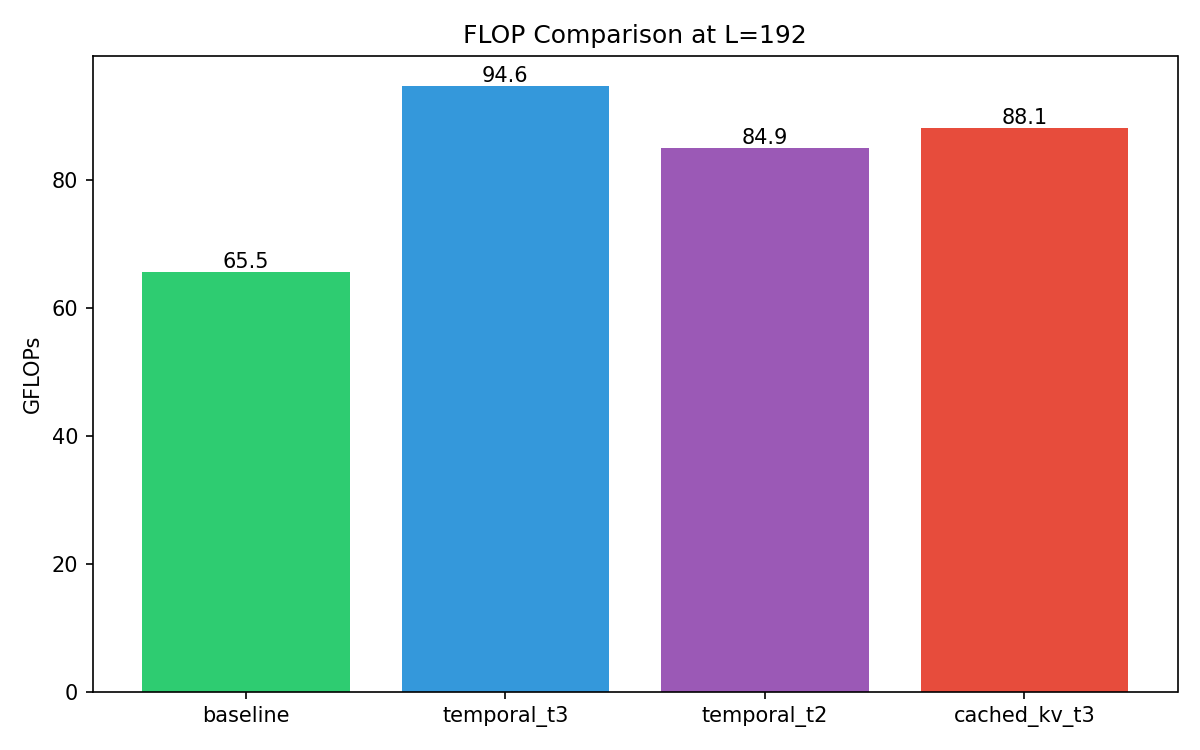
\includegraphics[width=\columnwidth]{figures/fig1_flop_comparison.png}
\caption{FLOP comparison across attention variants}
\label{fig:fig1_flop_comparison}
\end{figure}

\textit{Figure 1: FLOP comparison across attention variants. temporal\_t2 achieves 10.2\% reduction compared to temporal\_t3.}

\subsubsection{5.3 H-M2: Convergence --- FAIL}

\begin{table}[htbp]
\centering
\resizebox{\columnwidth}{!}{%
\begin{tabular}{lll}
\toprule
Metric & Expected & Actual \\
\midrule
Entropy Step 1 & Reference & 4.099 \\
Entropy Step 2 & < 4.099 & 4.139 \\
Entropy Change & > 5\% decrease & 0.98\% increase \\
Convergence Rate & Positive & -0.0098 \\
\bottomrule
\end{tabular}
}
\end{table}

Attention entropy increases across temporal steps, contradicting the convergence hypothesis. The mechanism was tested on a randomly-initialized model; trained weights may exhibit different behavior, but this was not tested.

\begin{figure}[htbp]
\centering
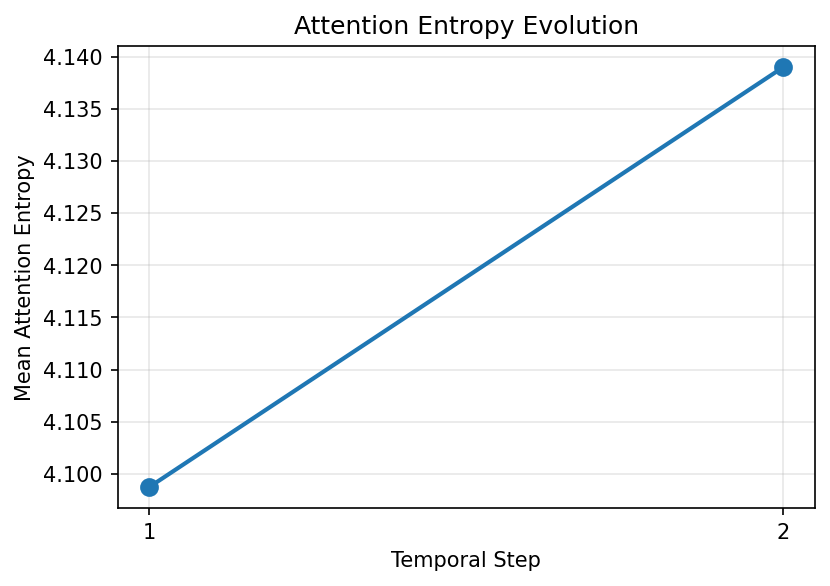
\includegraphics[width=\columnwidth]{figures/entropy_curve.png}
\caption{Attention entropy across temporal steps}
\label{fig:entropy_curve}
\end{figure}

\textit{Figure 2: Attention entropy increases across temporal steps rather than decreasing.}

\subsubsection{5.4 H-C1: Scaling --- FAIL}

\begin{table}[htbp]
\centering
\resizebox{\columnwidth}{!}{%
\begin{tabular}{llll}
\toprule
Seq Length & Baseline (T=3) GFLOPs & Proposed (T=2) GFLOPs & Reduction \\
\midrule
128 & 45.58 & 43.16 & 5.31\% \\
512 & 182.31 & 172.64 & 5.31\% \\
1024 & 364.62 & 345.27 & 5.31\% \\
\bottomrule
\end{tabular}
}
\end{table}

FLOP reduction is constant at 5.31\% across all sequence lengths. The scaling coefficient is 0.0. This follows from the FLOP formula: both variants scale as $T \times \text{seq\_len}^2$, so the ratio $T_{\text{proposed}}/T_{\text{baseline}} = 2/3$ is constant regardless of sequence length.

\begin{figure}[htbp]
\centering
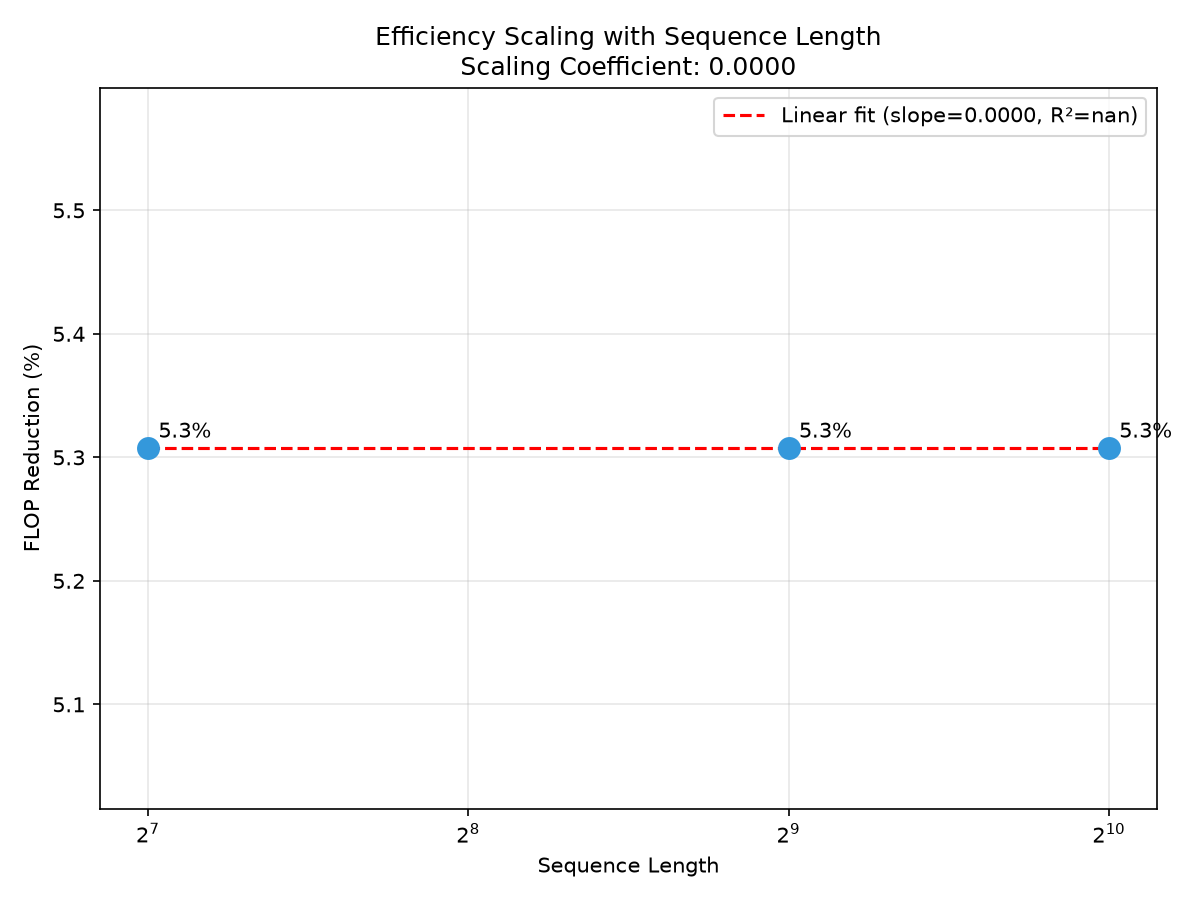
\includegraphics[width=\columnwidth]{figures/fig2_scaling_curve.png}
\caption{Scaling curve across sequence lengths}
\label{fig:fig2_scaling_curve}
\end{figure}

\textit{Figure 3: FLOP reduction is constant across sequence lengths.}

\subsubsection{5.5 Summary}

\begin{table}[htbp]
\centering
\resizebox{\columnwidth}{!}{%
\begin{tabular}{lll}
\toprule
Sub-Hypothesis & Gate & Status \\
\midrule
H-E1 Existence & MUST\_WORK & **PASS** \\
H-M1 Efficiency & MUST\_WORK & **PASS** \\
H-M2 Convergence & SHOULD\_WORK & **FAIL** \\
H-C1 Scaling & SHOULD\_WORK & **FAIL** \\
\bottomrule
\end{tabular}
}
\end{table}

